\documentclass[tikz,border=2pt,11pt]{standalone}
\usetikzlibrary{calc}
\usetikzlibrary{backgrounds}
\usetikzlibrary{positioning}
\usetikzlibrary{arrows.meta}
\usetikzlibrary{fit}
\usepackage{amsmath}
\usepackage{amssymb}
\usepackage{tikz}
\newcommand{\DoNotLoadEpstopdf}{}
\newcommand{\nCat}{n\mathrm{Cat}}
\newcommand{\omCat}{\omega\mathrm{Cat}}
\newcommand{\sSet}{\mathrm{sSet}}
\newcommand{\Street}{N_n}
\newcommand{\OrdN}{N}
\newcommand{\U}[1]{U_{#1}}
\newcommand{\Uinf}[1]{U^{\infty}_{#1}}
\newcommand{\Disk}[1]{D_{#1}}
\newcommand{\Orient}[1]{\mathcal O_{#1}}
\newcommand{\trunc}{\tau_n}
\newcommand{\Sd}{\mathrm{Sd}}
\newcommand{\Ex}{\mathrm{Ex}}
\newcommand{\id}{\mathrm{id}}
\DeclareMathOperator{\Hom}{Hom}
\DeclareMathOperator*{\colim}{colim}
\DeclareMathOperator{\Ob}{Ob}
\DeclareMathOperator{\im}{im}
\DeclareMathOperator{\sk}{sk}
\DeclareMathOperator{\dom}{dom}
\DeclareMathOperator{\cod}{cod}
\newcommand{\KQ}{\mathrm{KQ}}
\newcommand{\inj}{\text{-}\mathrm{inj}}
\newcommand{\cell}{\text{-}\mathrm{cell}}
\newcommand{\cof}{\text{-}\mathrm{cof}}
\begin{document}
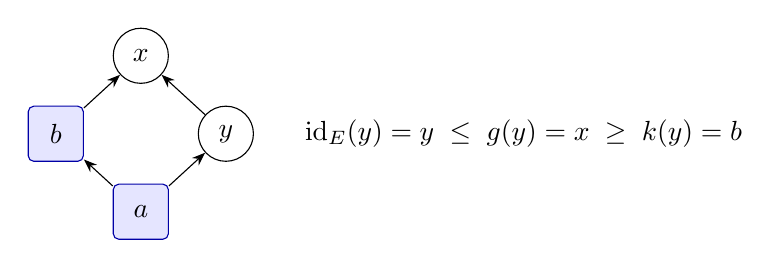
\begin{tikzpicture}[>=Stealth,scale=.9,
 old/.style={draw=blue!65!black,fill=blue!10,rounded corners=2pt,
             minimum width=7mm,minimum height=7mm},
 new/.style={draw,circle,minimum size=7mm}]
 \node[old] (a) at (0,0) {$a$};
 \node[old] (b) at (-1.2,1.1) {$b$};
 \node[new] (y) at (1.2,1.1) {$y$};
 \node[new] (x) at (0,2.2) {$x$};
 \draw[->] (a)--(b);
 \draw[->] (a)--(y);
 \draw[->] (b)--(x);
 \draw[->] (y)--(x);
 \node at (5.4,1.1)
   {$\id_E(y)=y\;\le\;g(y)=x\;\ge\;k(y)=b$};
\end{tikzpicture}
\end{document}
